% !TEX program = xelatex
\documentclass[UTF8,a4paper,12pt]{ctexart}

\usepackage[a4paper,margin=2.2cm]{geometry}
\usepackage{graphicx}
\usepackage{booktabs}
\usepackage{float}
\usepackage{subcaption}
\usepackage{caption}
\usepackage{array}
\usepackage{threeparttable}
\usepackage{longtable}
\usepackage{multirow}
\usepackage{hyperref}

\captionsetup{font=small,labelfont=bf}
\graphicspath{{figures/}}
\hypersetup{
  colorlinks=true,
  linkcolor=black,
  citecolor=black,
  urlcolor=black
}

\title{气体传感器分类实验结果展示}
\author{}
\date{}

\begin{document}

\maketitle

\begin{abstract}
本文围绕 \textit{Gas Sensor Array Drift at Different Concentrations} 数据集开展气体分类实验展示。所有实验均采用固定且非随机的数据划分方式：在每个类别内部保持原始样本顺序，并按照 $60\%/20\%/20\%$ 划分训练集、验证集和测试集。本文汇总展示了传统机器学习模型、深度学习基线模型、最终改进模型以及复杂度对比结果，并给出与之对应的可视化图表，便于直接用于课程论文或 Overleaf 排版。
\end{abstract}

\textbf{关键词：}气体传感器；固定划分；传统机器学习；深度学习；可视化

\section{实验设置}

本文使用 UCI 数据集 \textit{Gas Sensor Array Drift at Different Concentrations}。数据集共包含 13910 个样本、128 维传感器特征和 6 个气体类别。为避免随机划分带来的结果波动，本文采用严格固定的训练集、验证集和测试集划分方式：在每个类别内部保持原始样本顺序，依次取前 $60\%$ 作为训练集，中间 $20\%$ 作为验证集，最后 $20\%$ 作为测试集。最终得到训练集 8343 个样本、验证集 2782 个样本、测试集 2785 个样本。本文统一采用 Accuracy、Macro-F1 和 Balanced Accuracy 作为主要评价指标，其中 Macro-F1 作为核心指标。

\section{传统机器学习结果}

\begin{table}[H]
\centering
\caption{传统机器学习模型测试结果对比}
\label{tab:traditional}
\begin{threeparttable}
\setlength{\tabcolsep}{7pt}
\begin{tabular}{lcccc}
\toprule
模型 & 验证集 Macro-F1 & 测试集 Macro-F1 & 测试集 Accuracy & 测试集 Balanced Accuracy \\
\midrule
Extra Trees & 0.7798 & \textbf{0.6921} & 0.6908 & \textbf{0.7210} \\
Logistic Regression & 0.7875 & 0.6911 & \textbf{0.6998} & 0.7200 \\
SVM (RBF) & \textbf{0.7933} & 0.6739 & 0.6707 & 0.7022 \\
Random Forest & 0.7585 & 0.6471 & 0.6488 & 0.6774 \\
kNN & 0.7371 & 0.6317 & 0.6338 & 0.6633 \\
\bottomrule
\end{tabular}
\begin{tablenotes}[flushleft]
\footnotesize
\item 注：加粗结果表示该列最优值。
\end{tablenotes}
\end{threeparttable}
\end{table}

由表 \ref{tab:traditional} 可见，在传统机器学习模型中，Extra Trees 在测试集 Macro-F1 和 Balanced Accuracy 两项指标上均取得最优结果，说明树模型对当前固定划分下的类别边界具有较好的适应能力；Logistic Regression 的测试集 Accuracy 最高，表现出较强的整体判别稳定性；SVM (RBF) 在验证集上表现最好，但测试集下降更明显，说明其对顺序漂移更为敏感。

\begin{figure}[H]
\centering
\begin{subfigure}[b]{0.48\textwidth}
  \centering
  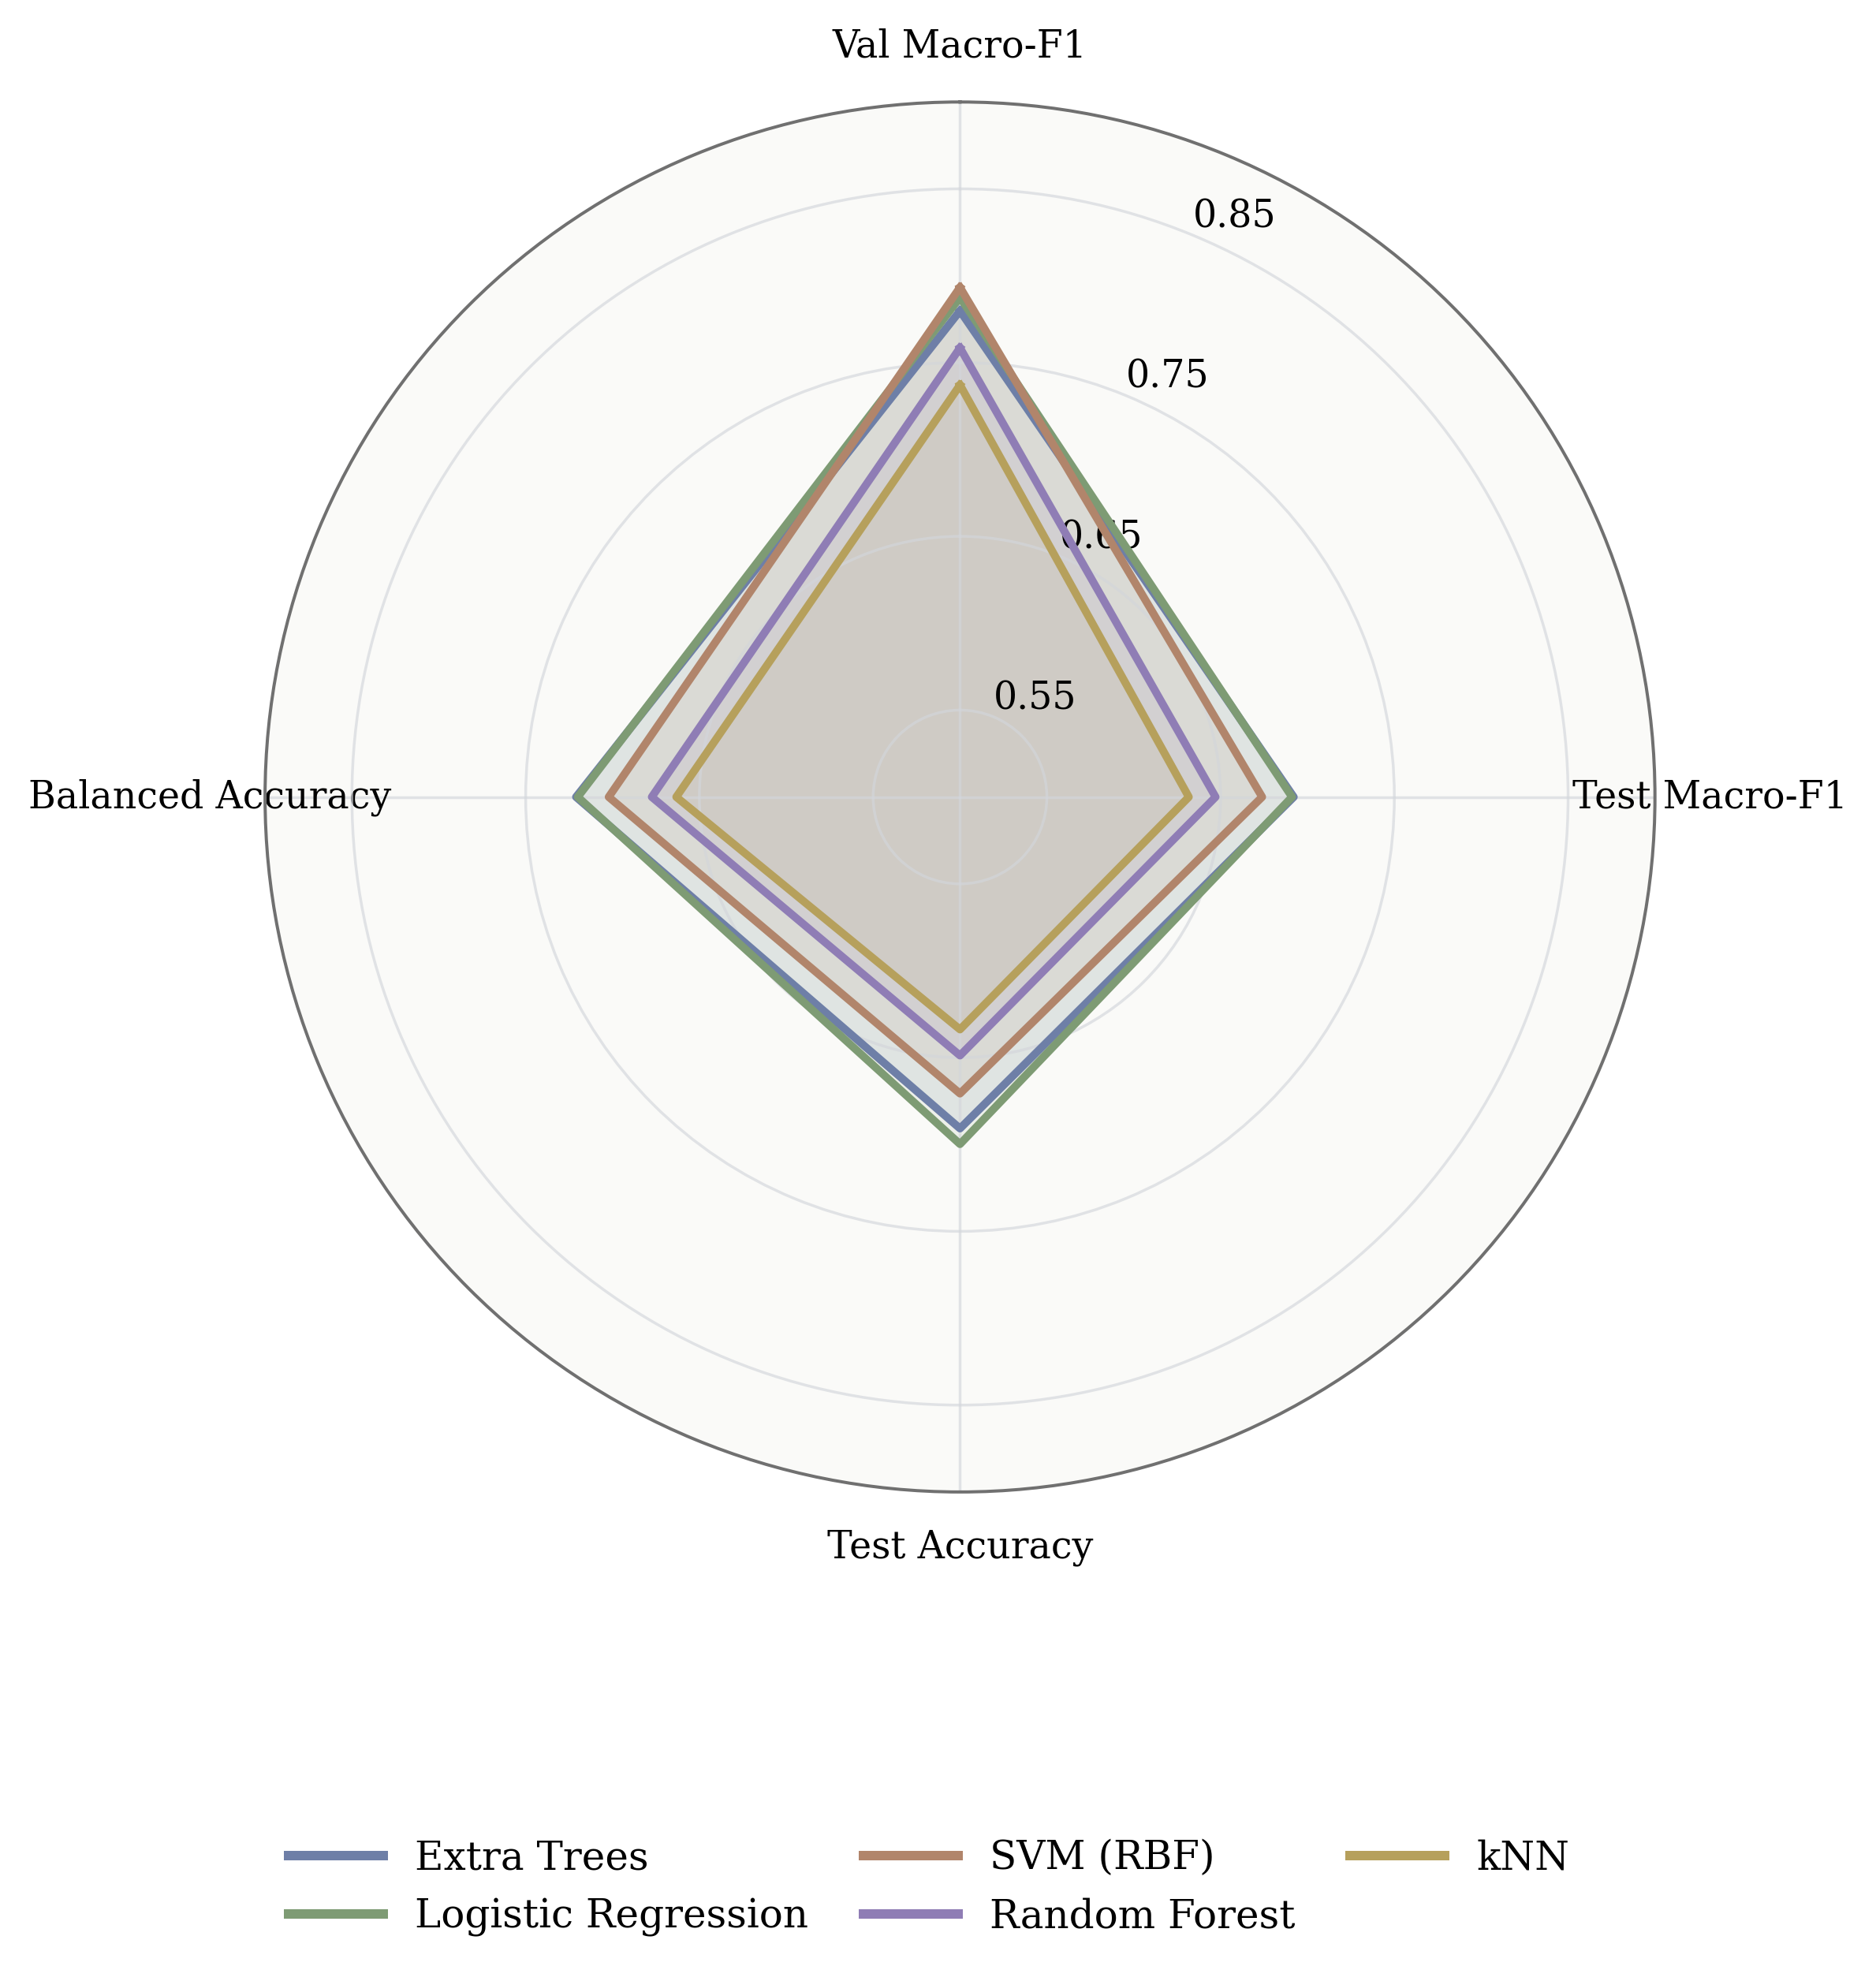
\includegraphics[width=\linewidth]{traditional_models_radar.png}
  \caption{传统机器学习模型雷达图}
\end{subfigure}
\hfill
\begin{subfigure}[b]{0.48\textwidth}
  \centering
  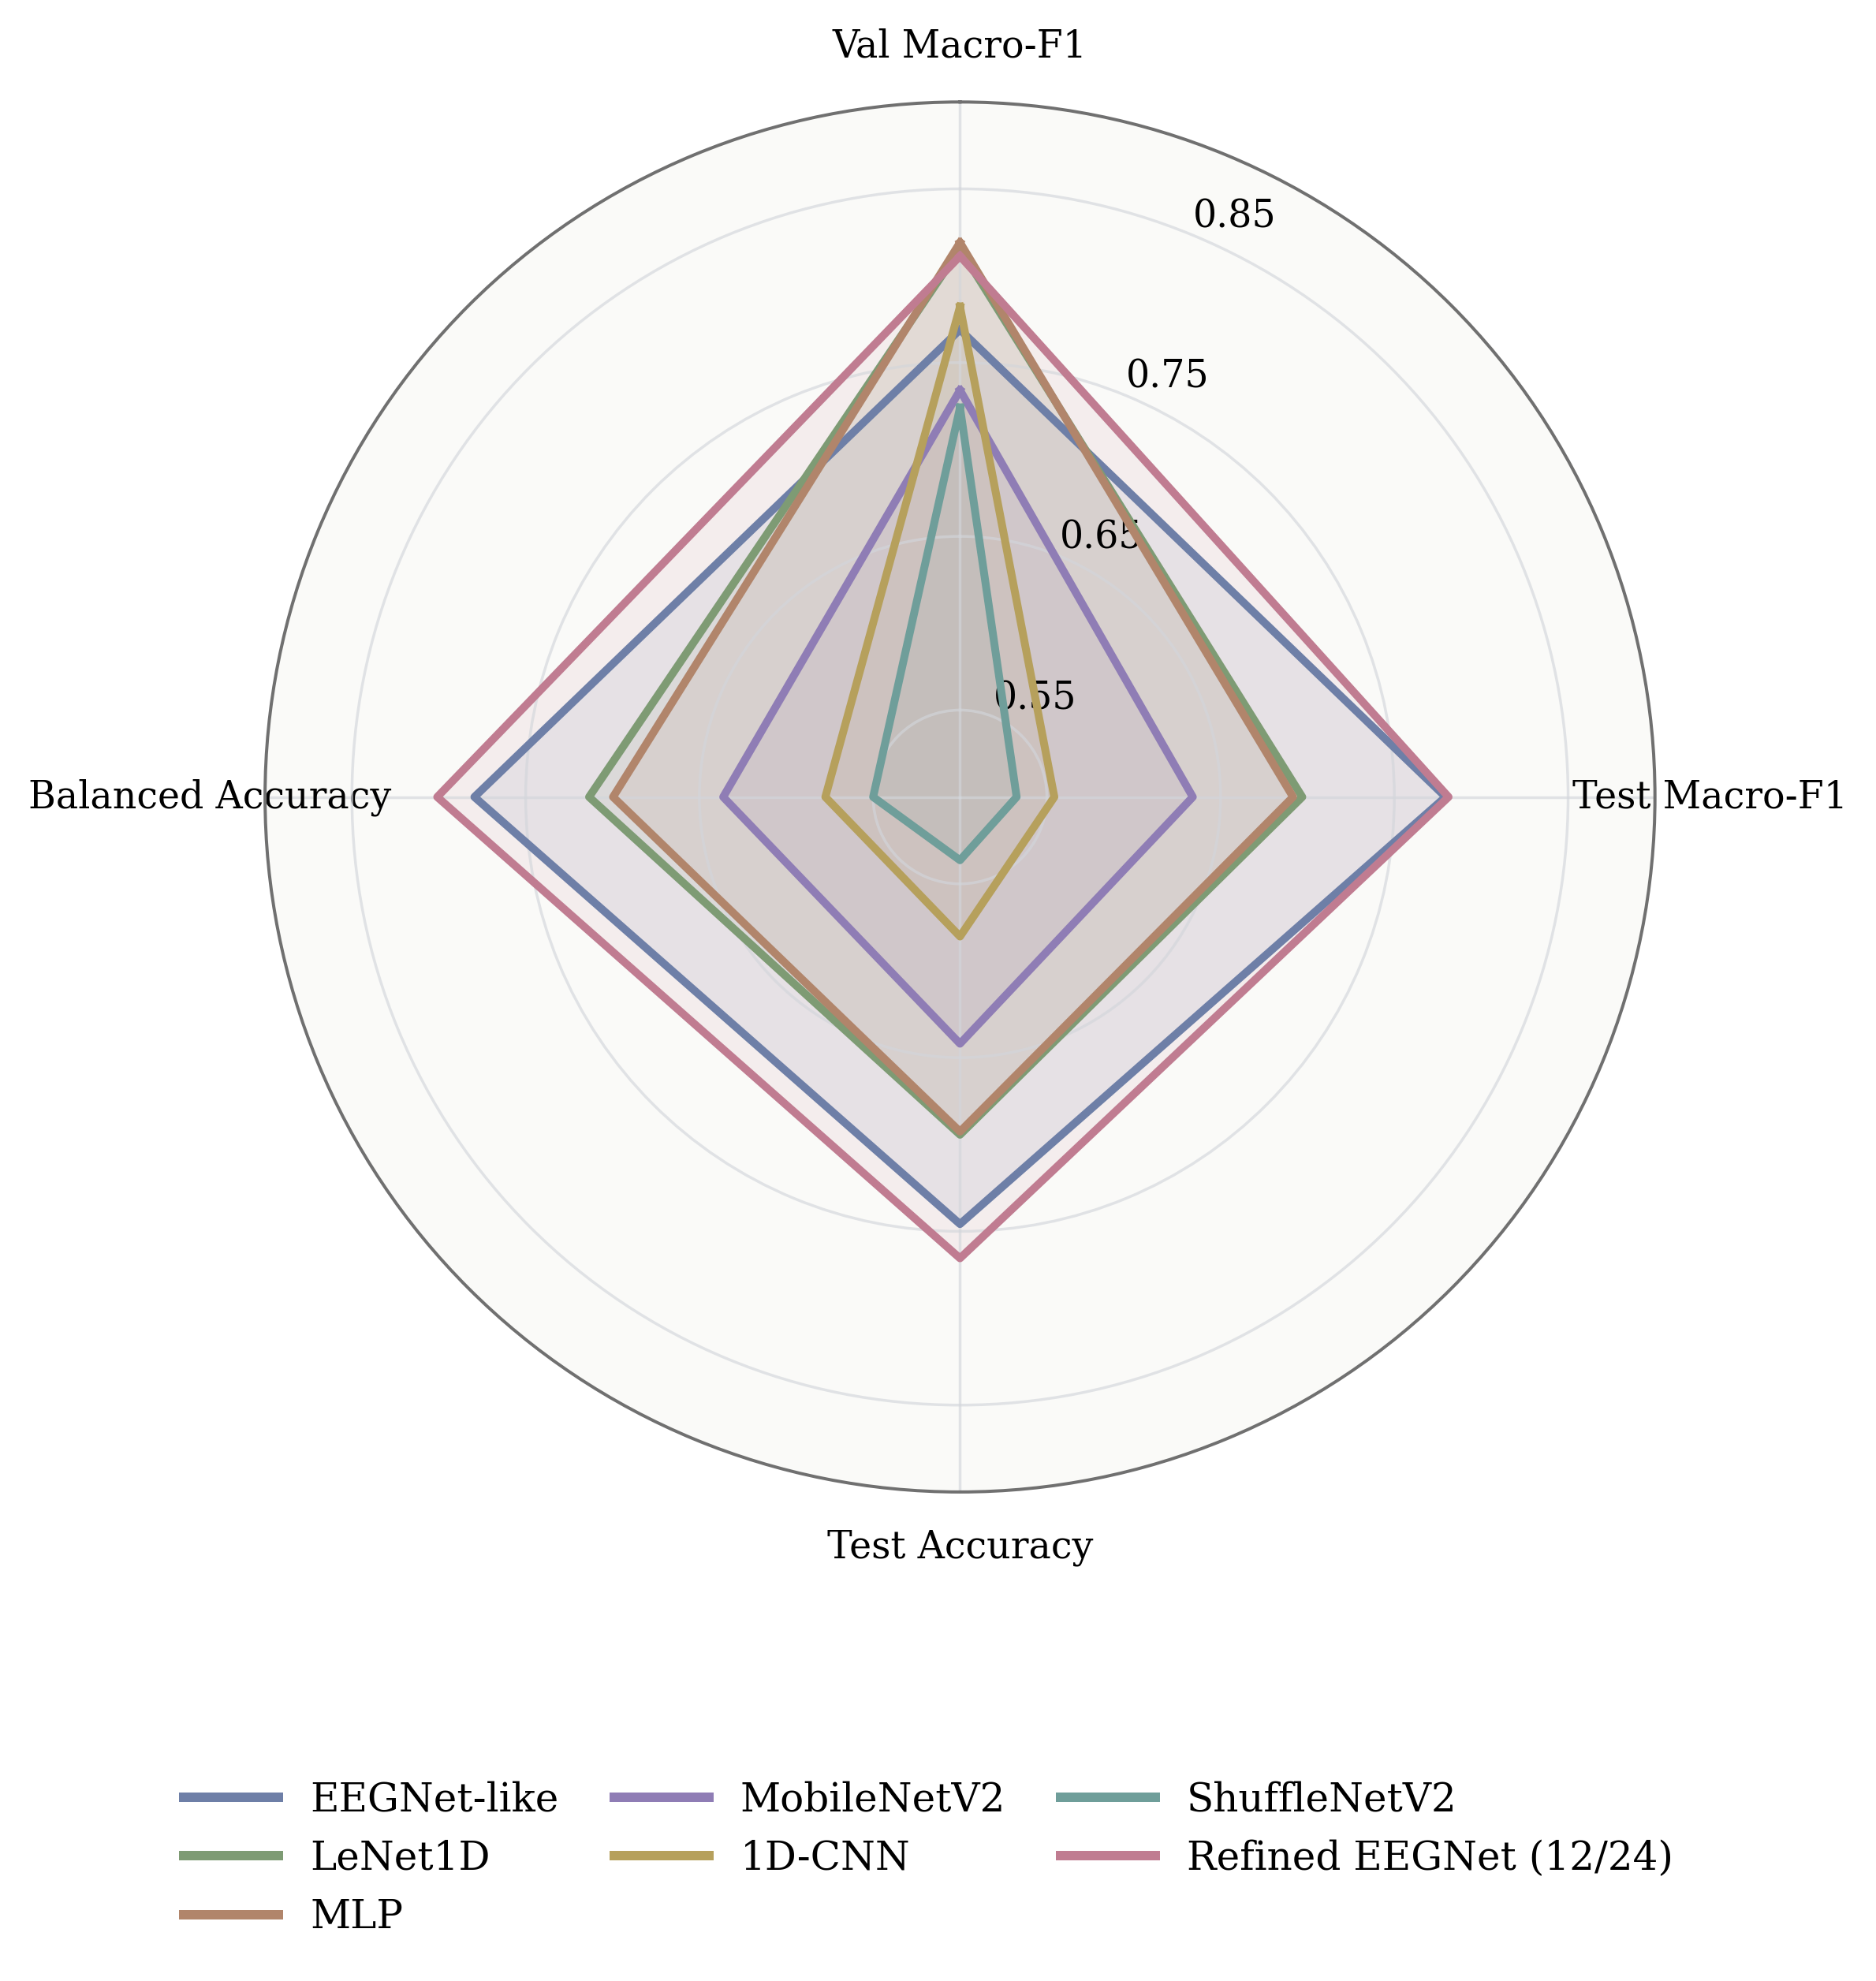
\includegraphics[width=\linewidth]{deep_models_radar.png}
  \caption{深度学习基线模型雷达图}
\end{subfigure}
\caption{传统机器学习模型与深度学习基线模型的综合性能雷达图}
\label{fig:radar-main}
\end{figure}

\section{深度学习基线结果}

\begin{table}[H]
\centering
\caption{深度学习基线模型测试结果对比}
\label{tab:deep}
\begin{threeparttable}
\setlength{\tabcolsep}{7pt}
\begin{tabular}{lcccc}
\toprule
模型 & 验证集 Macro-F1 & 测试集 Macro-F1 & 测试集 Accuracy & 测试集 Balanced Accuracy \\
\midrule
EEGNet-like & 0.7690 & \textbf{0.7795} & \textbf{0.7458} & \textbf{0.7795} \\
LeNet1D & 0.8155 & 0.6970 & 0.6944 & 0.7135 \\
MLP & \textbf{0.8191} & 0.6917 & 0.6926 & 0.6997 \\
MobileNetV2 & 0.7341 & 0.6340 & 0.6420 & 0.6363 \\
1D-CNN & 0.7822 & 0.5543 & 0.5803 & 0.5775 \\
ShuffleNetV2 & 0.7241 & 0.5326 & 0.5364 & 0.5500 \\
\bottomrule
\end{tabular}
\begin{tablenotes}[flushleft]
\footnotesize
\item 注：加粗结果表示该列最优值。
\end{tablenotes}
\end{threeparttable}
\end{table}

从表 \ref{tab:deep} 可以看出，EEGNet-like 在深度学习基线中显著优于其他网络结构，在测试集 Macro-F1、Accuracy 和 Balanced Accuracy 三项指标上均取得最优结果。该结果说明，针对多通道传感器阵列设计的轻量结构比直接迁移通用卷积网络更适合当前任务。LeNet1D 和 MLP 虽然在验证集上具有一定竞争力，但在测试集上的泛化能力弱于 EEGNet-like。

\section{最终模型与代表性基线对比}

\begin{table}[H]
\centering
\caption{最终模型与代表性基线模型结果对比}
\label{tab:final}
\begin{threeparttable}
\setlength{\tabcolsep}{8pt}
\begin{tabular}{lcccc}
\toprule
模型 & 验证集 Macro-F1 & 测试集 Macro-F1 & 测试集 Accuracy & 测试集 Balanced Accuracy \\
\midrule
最佳传统模型（Extra Trees） & 0.7798 & 0.6921 & 0.6908 & 0.7210 \\
深度学习基线（EEGNet-like） & 0.7690 & 0.7795 & 0.7458 & 0.7795 \\
最终模型（Refined EEGNet (12/24)） & \textbf{0.8113} & \textbf{0.7812} & \textbf{0.7655} & \textbf{0.8009} \\
\bottomrule
\end{tabular}
\begin{tablenotes}[flushleft]
\footnotesize
\item 注：加粗结果表示该列最优值。
\end{tablenotes}
\end{threeparttable}
\end{table}

表 \ref{tab:final} 给出了本文最终模型与两类代表性基线模型的直接对比结果。与最佳传统模型相比，最终模型在测试集 Macro-F1 上提升了 0.0891，在测试集 Accuracy 上提升了 0.0747；与 EEGNet-like 深度学习基线相比，最终模型在测试集 Macro-F1 上进一步提升了 0.0017，在测试集 Accuracy 上提升了 0.0197，在 Balanced Accuracy 上提升了 0.0214。由此可见，最终模型在保持轻量化特征建模思路的同时，进一步增强了对不同类别气体的区分能力。

\begin{figure}[H]
\centering
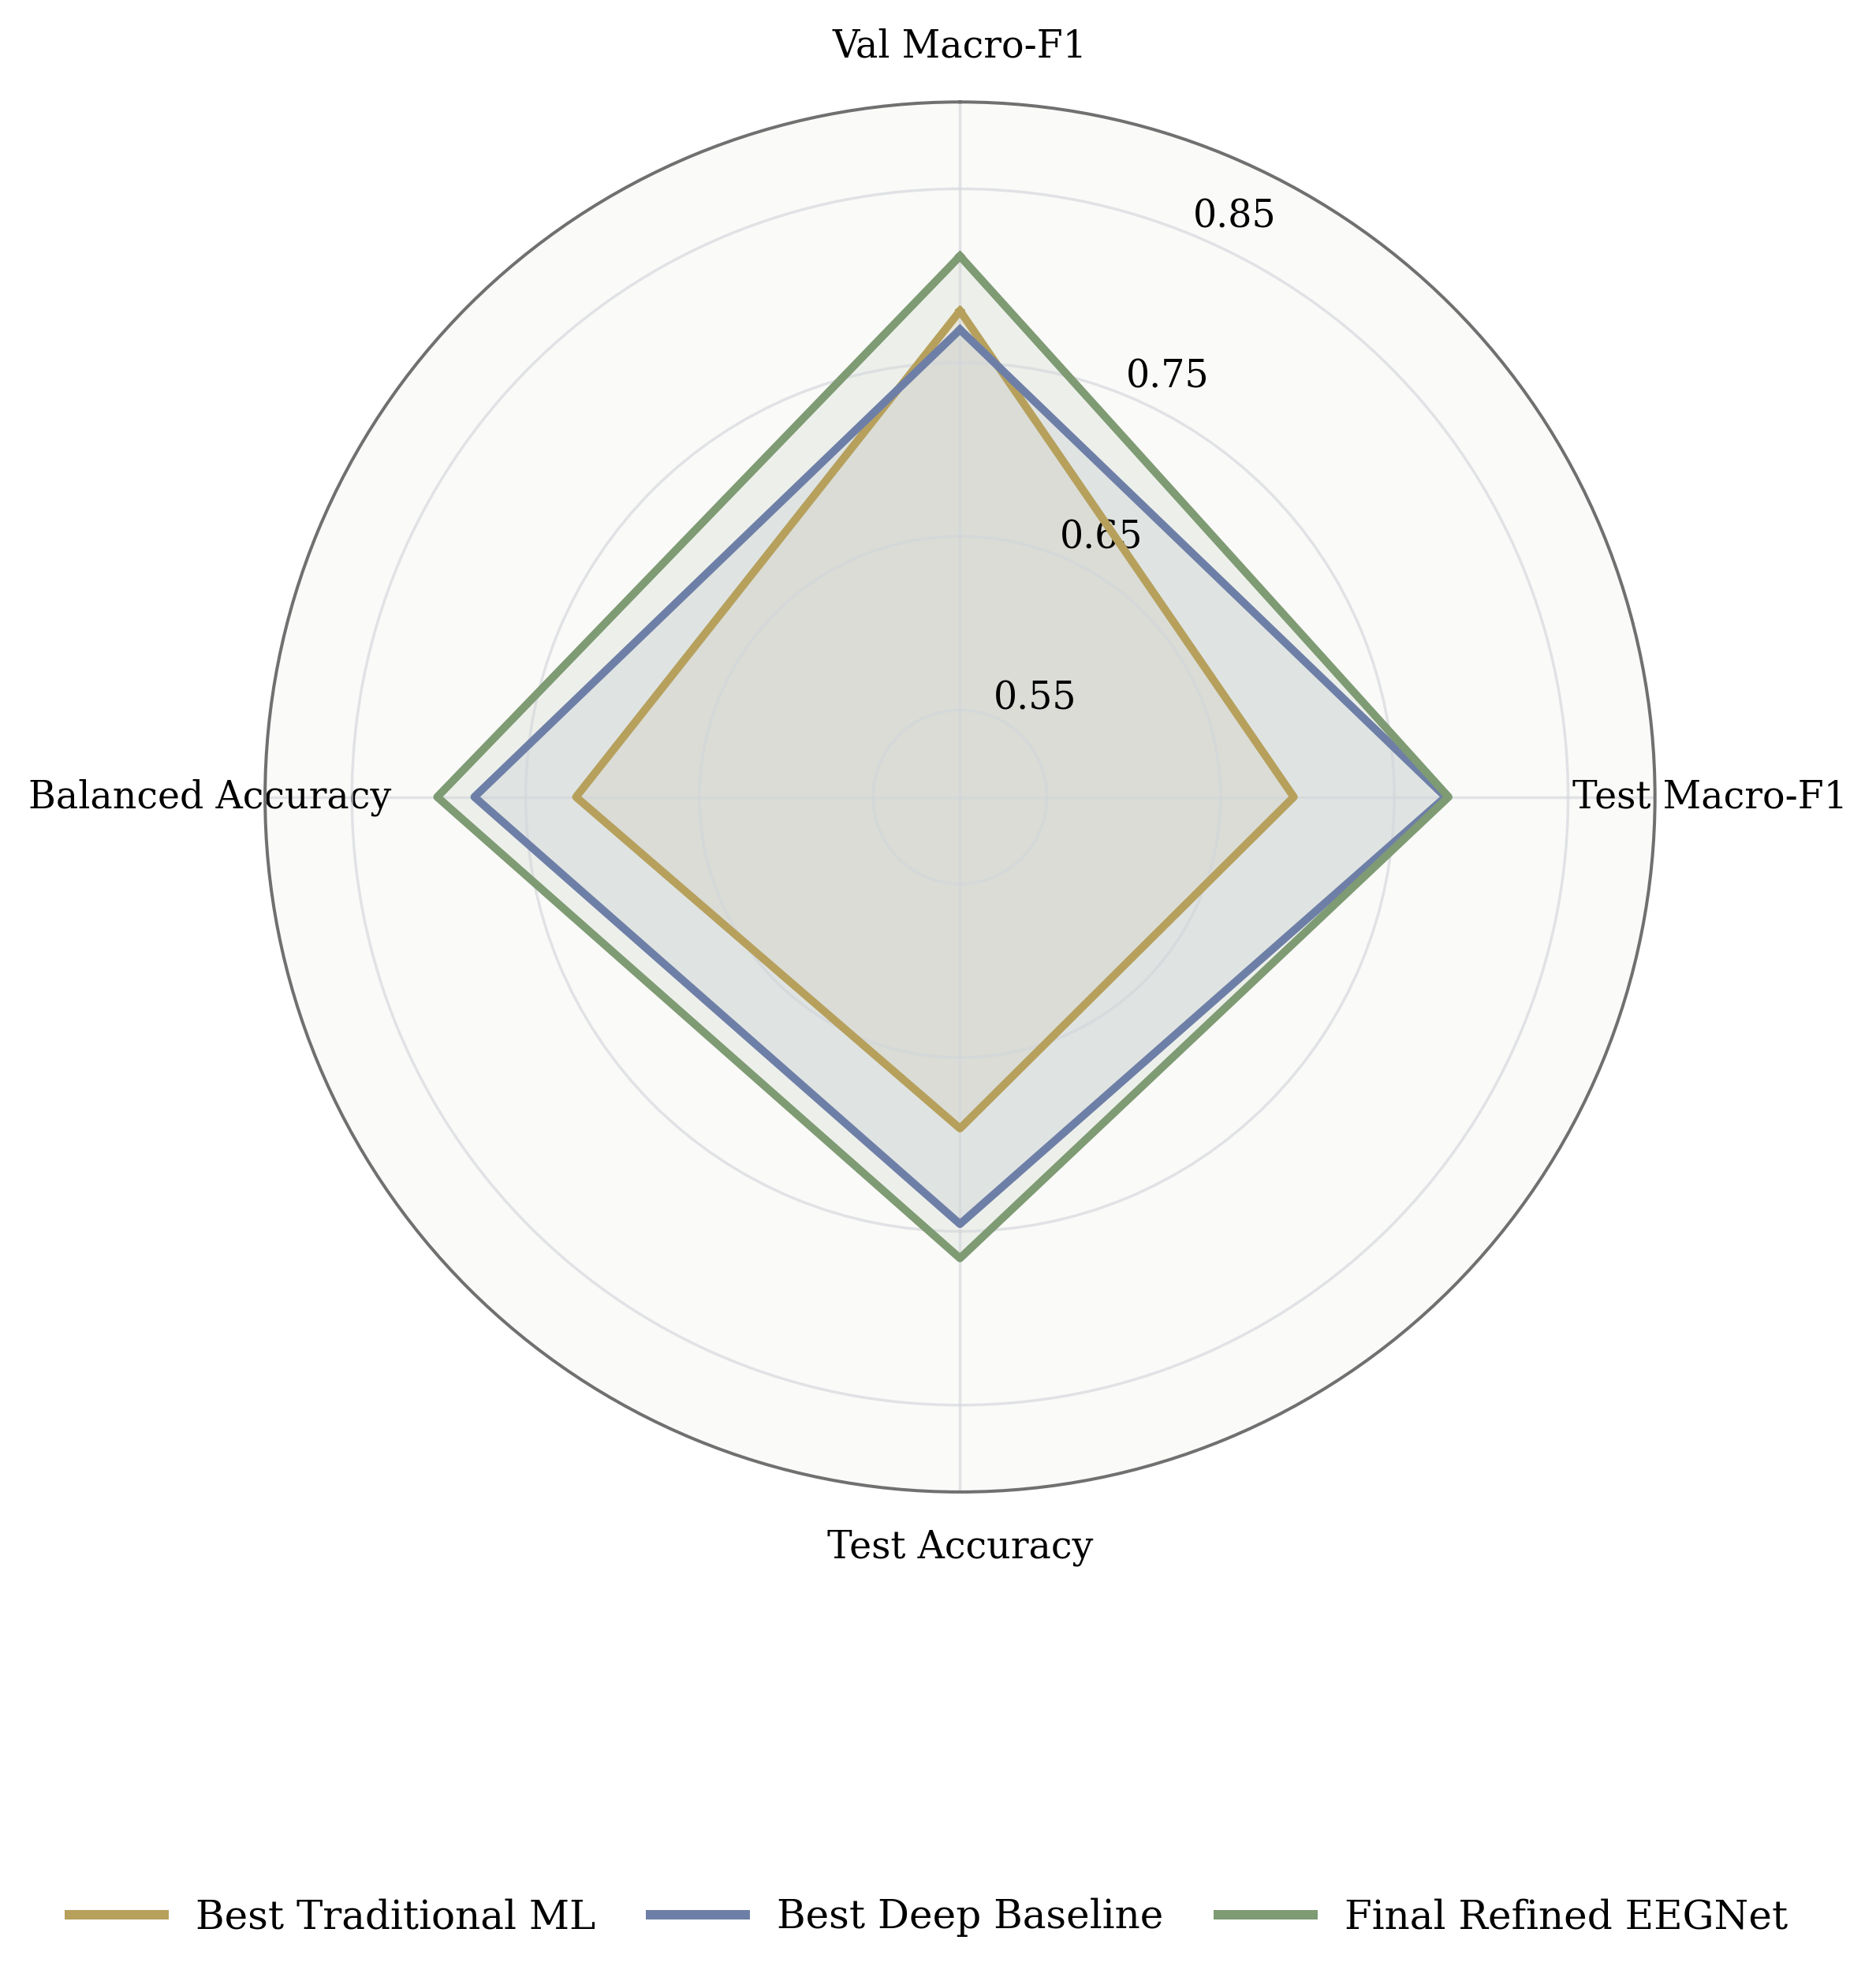
\includegraphics[width=0.78\linewidth]{winner_profile_radar.png}
\caption{最佳传统模型、最佳深度学习基线与最终模型的综合指标对比}
\label{fig:winner-radar}
\end{figure}

\begin{figure}[H]
\centering
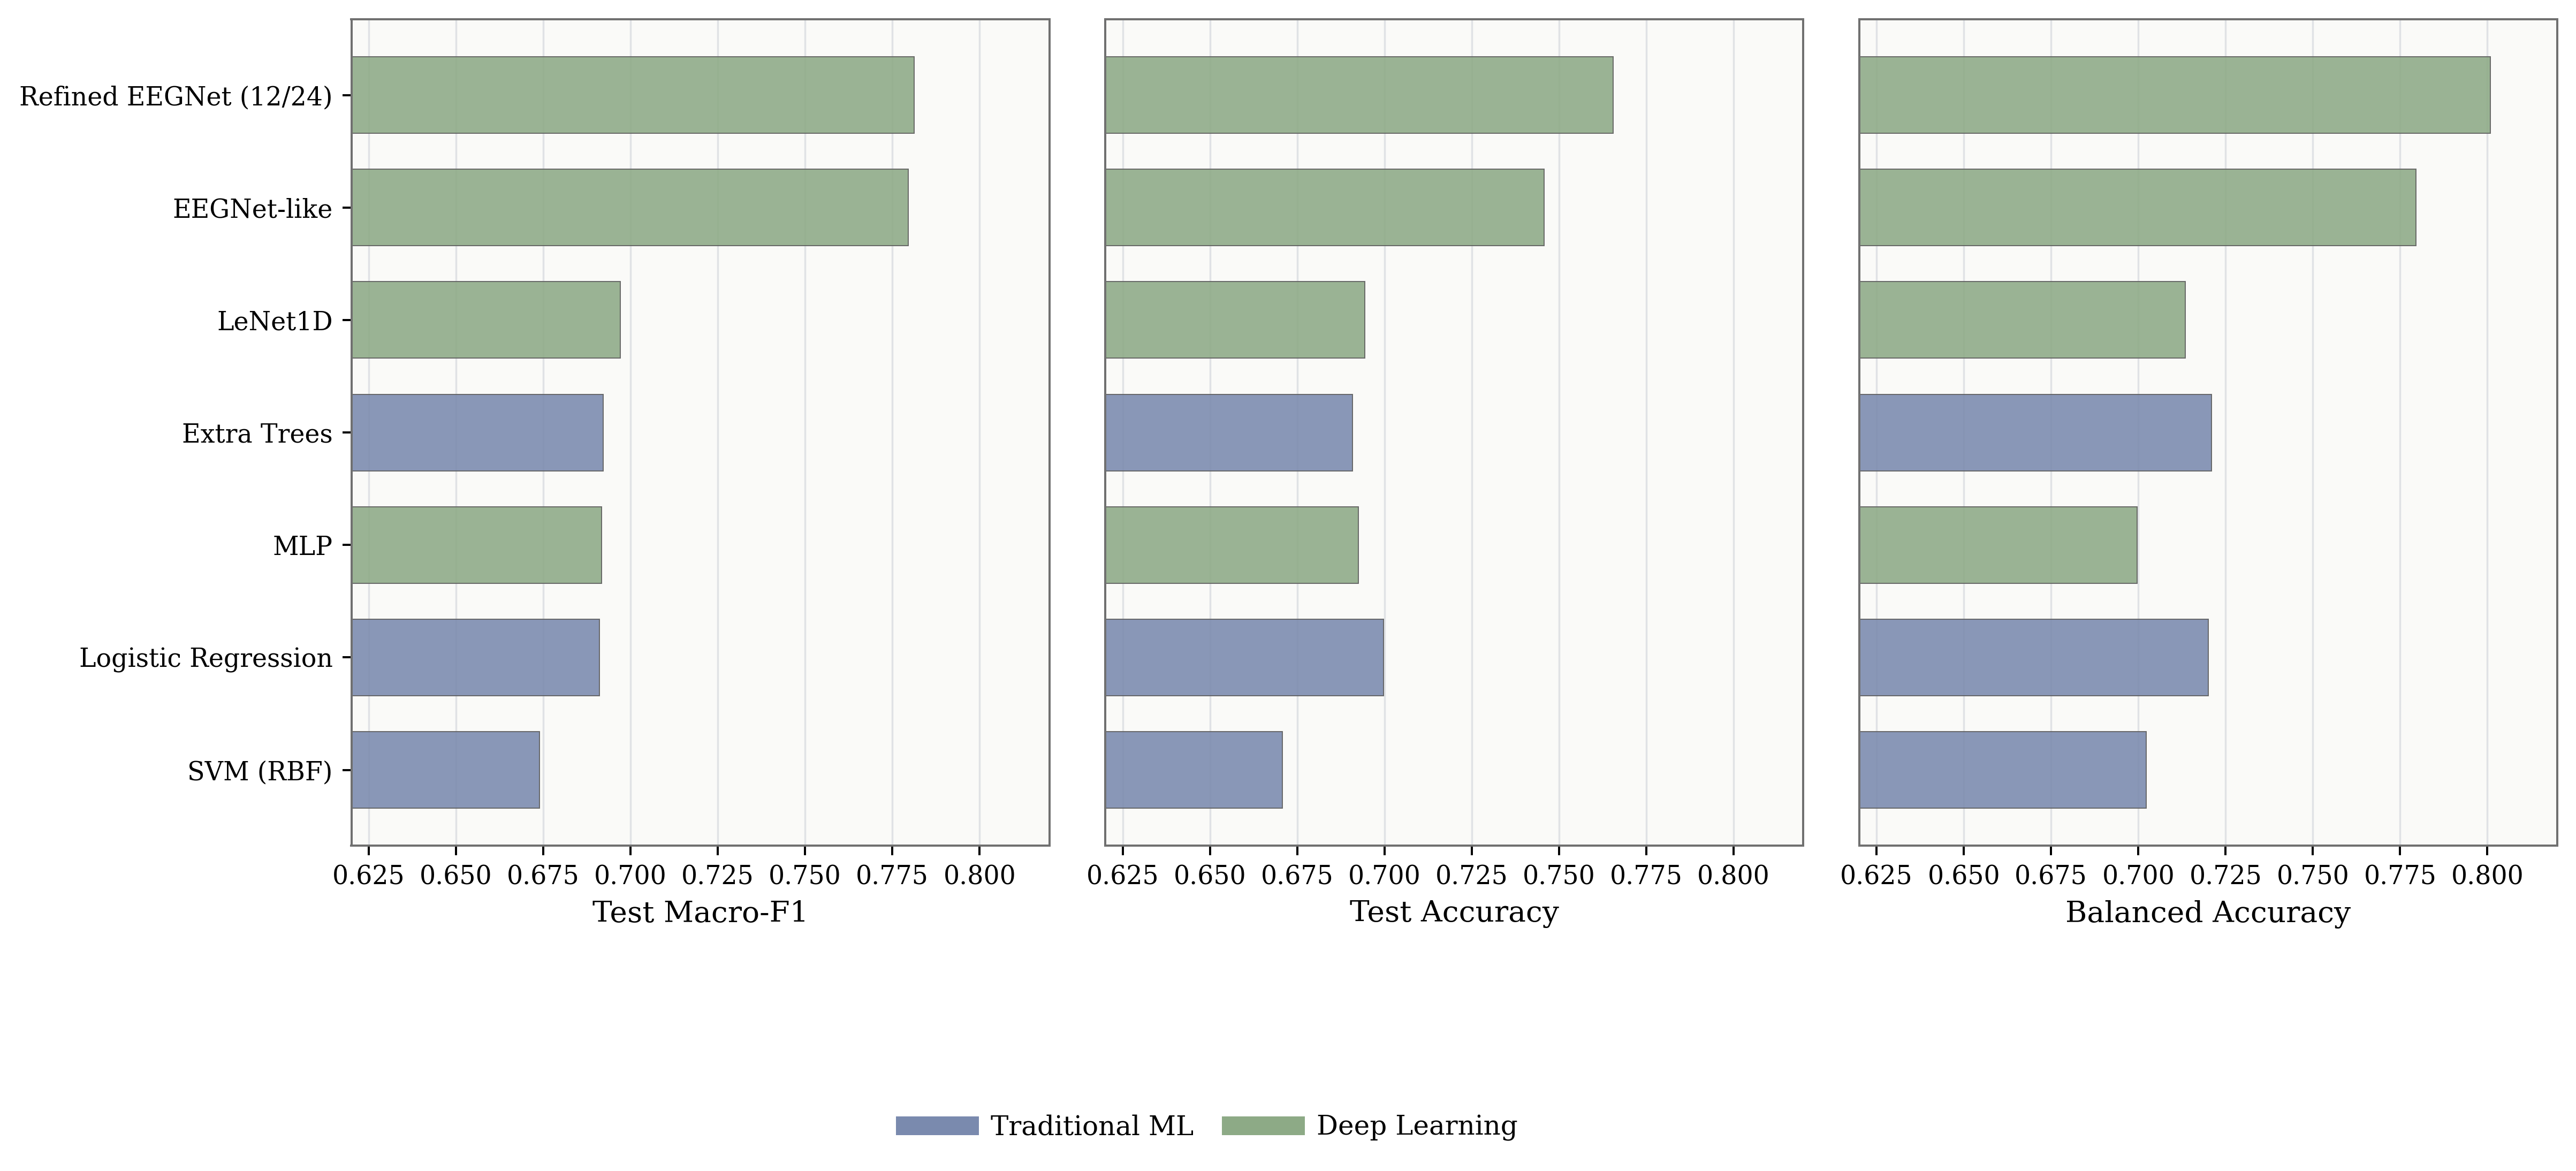
\includegraphics[width=\linewidth]{overall_selected_models_panels_2d.png}
\caption{代表性模型在测试集上的二维分面柱状对比图。三幅子图从左至右依次展示 Test Macro-F1、Test Accuracy 和 Balanced Accuracy。}
\label{fig:bars-panels}
\end{figure}

图 \ref{fig:bars-panels} 以二维分面方式对代表性模型进行了并列展示。与三维图形相比，该形式能够更直接地呈现不同模型在三个核心指标上的相对高低关系。可以看到，最终模型在三个子图中均位于前列，尤其在 Test Accuracy 与 Balanced Accuracy 上相较基线模型具有更明显优势，而最佳传统模型依然保持了较强的竞争力。

\section{特征空间可视化分析}

\begin{figure}[H]
\centering
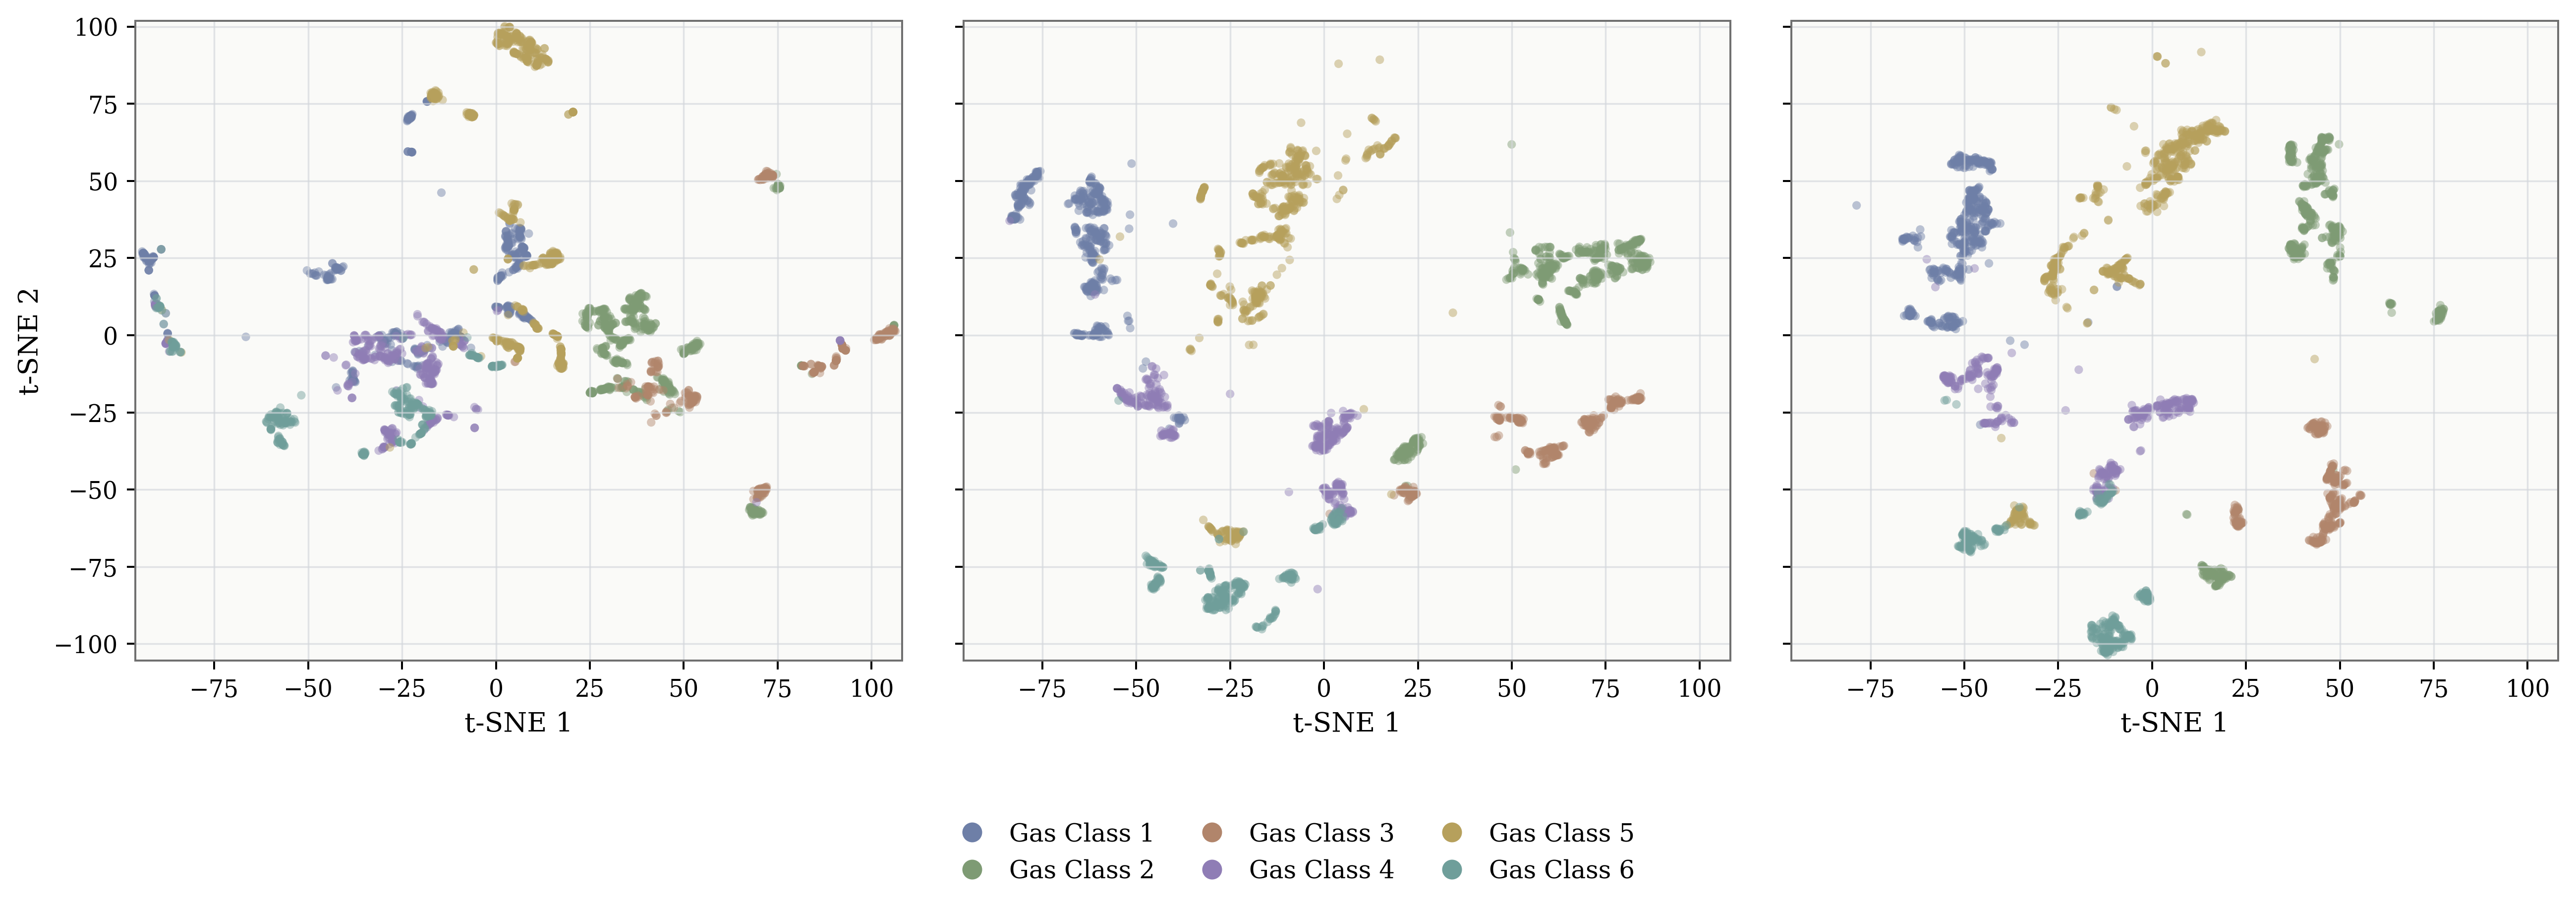
\includegraphics[width=\linewidth]{tsne_response_space_panels_2d.png}
\caption{三组代表性模型在测试集响应空间上的二维 t-SNE 可视化。三幅子图从左至右依次对应最佳传统模型、EEGNet-like 基线和最终模型。}
\label{fig:tsne}
\end{figure}

图 \ref{fig:tsne} 展示了三组代表性模型在测试集响应空间中的二维 t-SNE 投影结果。整体来看，最终模型对应的类别簇分布更紧凑、类间边界更清晰，尤其在若干易混类别之间表现出更明显的分离趋势；EEGNet-like 基线已经能够形成较稳定的类别簇，但仍存在局部交叠区域；最佳传统模型虽然同样具备一定的类别可分性，但簇结构相对更分散，反映出其高层表征能力弱于最终深度模型。

\section{精度与复杂度对比}

\begin{figure}[H]
\centering
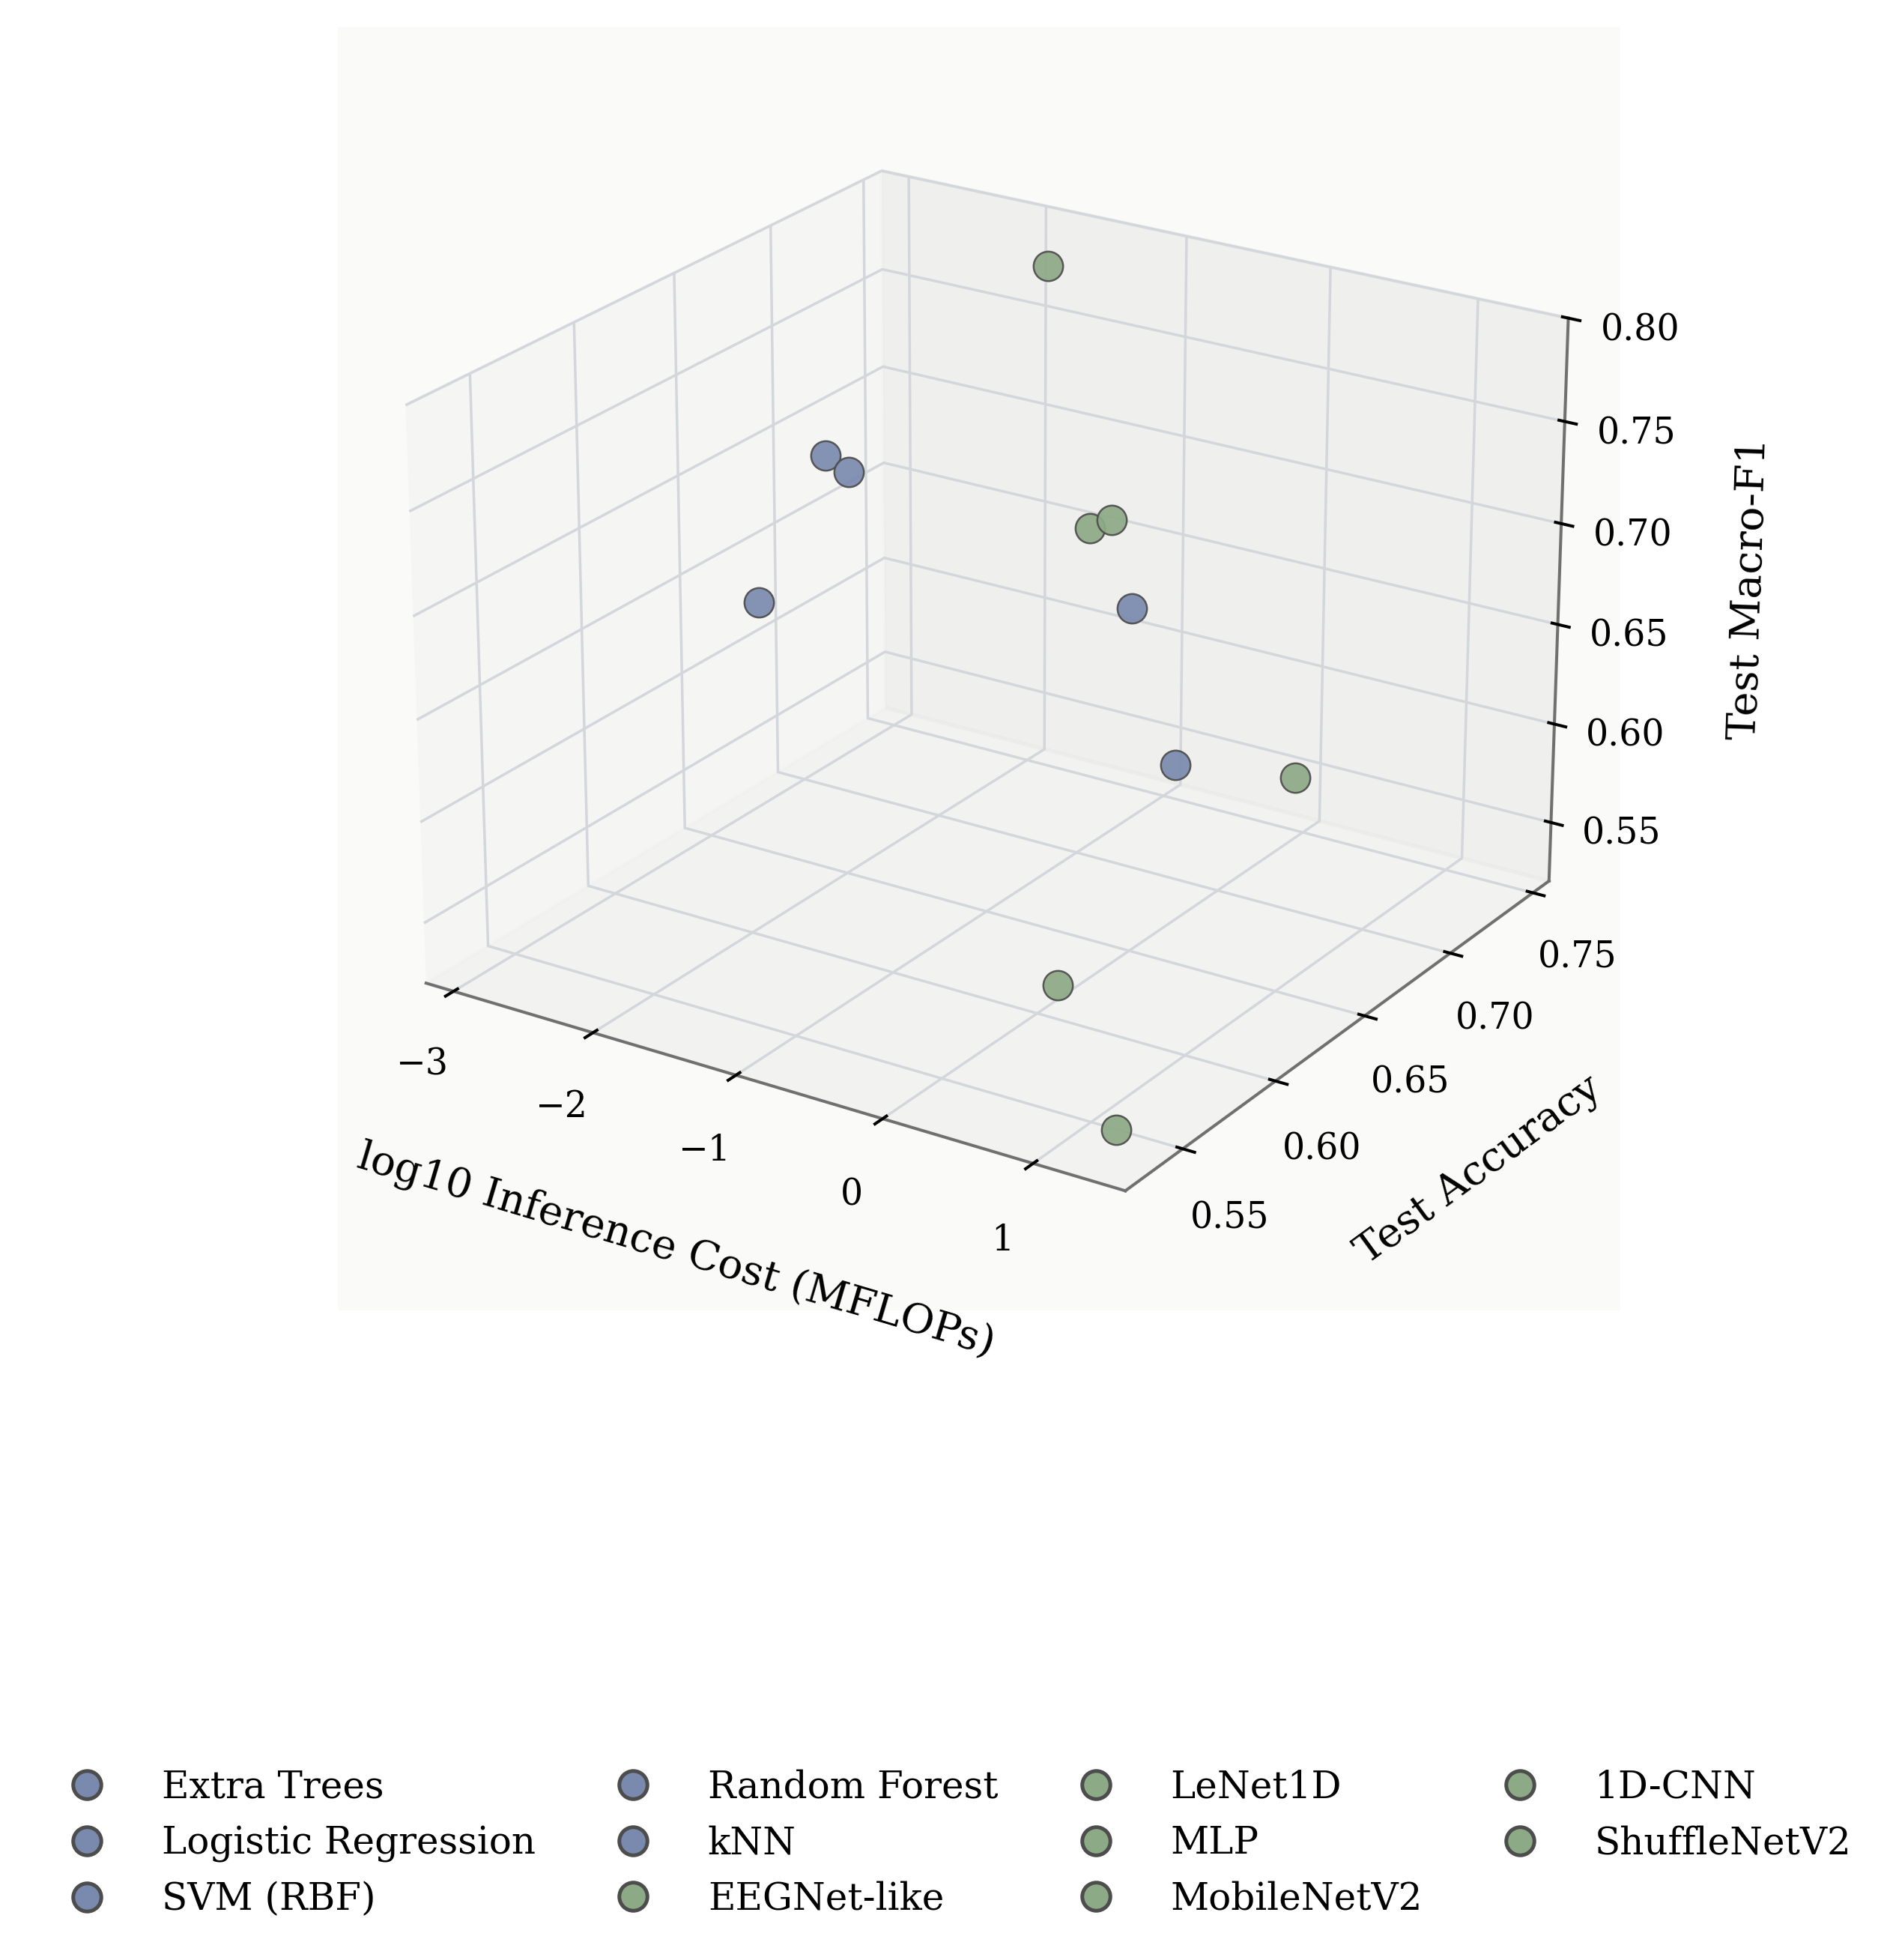
\includegraphics[width=0.84\linewidth]{efficiency_tradeoff_3d_scatter.png}
\caption{传统模型与深度学习模型的精度--复杂度三维散点图}
\label{fig:efficiency}
\end{figure}

\begin{table}[H]
\centering
\caption{代表性模型单样本推理复杂度对比}
\label{tab:complexity}
\begin{threeparttable}
\setlength{\tabcolsep}{6pt}
\begin{tabular}{llcc}
\toprule
类别 & 模型 & 单样本 MFLOPs / Ops & 参数量 \\
\midrule
传统机器学习 & Logistic Regression & \textbf{0.001536} & --- \\
传统机器学习 & Extra Trees & 0.003005 & --- \\
传统机器学习 & Random Forest & 0.002490 & --- \\
传统机器学习 & SVM (RBF) & 0.554415 & --- \\
传统机器学习 & kNN & 3.195369 & --- \\
\midrule
深度学习 & EEGNet-like & \textbf{0.015718} & \textbf{766} \\
深度学习 & MLP & 0.149894 & 75,334 \\
深度学习 & LeNet1D & 0.201078 & 67,006 \\
深度学习 & 1D-CNN & 2.459142 & 32,326 \\
深度学习 & MobileNetV2 & 15.940870 & 695,078 \\
深度学习 & ShuffleNetV2 & 21.626886 & 347,510 \\
\bottomrule
\end{tabular}
\begin{tablenotes}[flushleft]
\footnotesize
\item 注：表中加粗结果表示同类模型中的最小复杂度或最小参数规模。传统模型对应数值为推理阶段的近似计算代价。
\end{tablenotes}
\end{threeparttable}
\end{table}

图 \ref{fig:efficiency} 与表 \ref{tab:complexity} 共同表明，EEGNet-like 及其后续最终模型路线在当前任务中具备较好的精度--复杂度平衡。一方面，传统模型中的 Logistic Regression 与 Extra Trees 具有较低的推理代价，适合作为轻量化基线；另一方面，EEGNet-like 在深度学习模型中具有极低的计算开销和参数规模，同时仍能取得优于多数模型的测试性能，这为最终模型的进一步提升提供了坚实起点。

\section{结论}

综合以上结果可以得到以下结论。第一，在传统机器学习模型中，Extra Trees 是最强基线模型，测试集 Macro-F1 达到 0.6921。第二，在深度学习基线模型中，EEGNet-like 具有最优的综合性能，测试集 Macro-F1 达到 0.7795。第三，最终模型 Refined EEGNet (12/24) 在验证集和测试集上均取得最优结果，测试集 Macro-F1 达到 0.7812，测试集 Accuracy 达到 0.7655，说明该模型在当前固定划分任务下具有最强的泛化表现。第四，从特征空间可视化与复杂度分析来看，最终模型不仅在分类性能上优于代表性基线，同时也保持了良好的结构紧凑性与工程可用性。

\end{document}
